% Нечётное продолжение начальных данных с полупрямой x >= 0 на всю ось.
% Сплошная линия -- исходные данные, пунктир -- продолжение.
\begin{figure}[htbp]
\centering
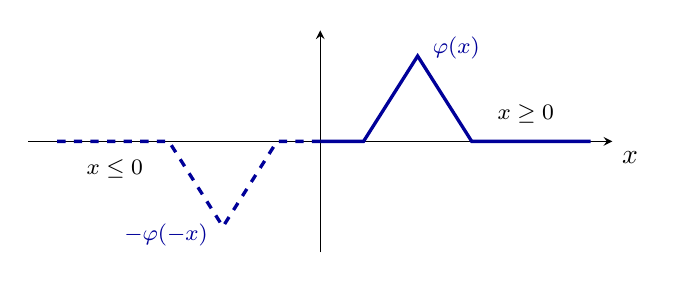
\begin{tikzpicture}
\begin{axis}[
  width=9cm, height=4.4cm,
  axis lines=middle,
  xmin=-2.7, xmax=2.7, ymin=-1.3, ymax=1.3,
  xlabel={$x$},
  xlabel style={anchor=north west},
  xtick=\empty, ytick=\empty, clip=false,
]
  % исходные данные на x >= 0
  \addplot[very thick, blue!60!black]
    coordinates {(0,0) (0.4,0) (0.9,1) (1.4,0) (2.5,0)};
  % нечётное продолжение на x <= 0
  \addplot[very thick, blue!60!black, dashed]
    coordinates {(0,0) (-0.4,0) (-0.9,-1) (-1.4,0) (-2.5,0)};

  \node[blue!60!black, anchor=south west, font=\footnotesize] at (axis cs:0.95,0.85)
    {$\varphi(x)$};
  \node[blue!60!black, anchor=north east, font=\footnotesize] at (axis cs:-0.95,-0.85)
    {$-\varphi(-x)$};
  \node[anchor=south, font=\footnotesize] at (axis cs:1.9,0.1) {$x \ge 0$};
  \node[anchor=north, font=\footnotesize] at (axis cs:-1.9,-0.1) {$x \le 0$};
\end{axis}
\end{tikzpicture}
\caption{Нечётное продолжение $\Phi$ данных $\varphi$ с полупрямой на всю ось.
Нечётность гарантирует $\Phi(0) = 0$, а вместе с ней и условие закрепления
$u|_{x=0} = 0$ для решения, построенного по формуле Даламбера.}
\label{fig:odd-extension}
\end{figure}
